In the forthcoming deployment of WebRTC systems, we speculate that high
quality\footnote{normally, high quality corresponds to an increase in required
bandwidth.} video conferencing will see wide-scale adoption. To assure
stability of the network (and avoid congestion collapse), these real-time
communication systems are required to implement some kind of congestion
control for their RTP-based media traffic.

RTP transmits the media data over IP using a variety of transport layer
protocols such as UDP, TCP, and Datagram Congestion Control Protocol (DCCP).
Consequently, congestion control for RTP-based media flows is implemented
either in the application or the media flows are transmitted over
congestion-controlled transport (TCP or DCCP). While using a congestion-controlled 
transport may be safe for the network, it is sub-optimal for the
media quality unless the congestion-controlled transport is designed to carry
media flows. Unfortunately, TCP is only suitable for interactive multimedia
for paths with very low RTT (<100\,\emph{ms} )~\cite{Brosh:tcp-real-time}, and
DCCP packets have problems with NAT traversal~\cite{schier:DCCP} unless DCCP is
encapsulated in UDP~\cite{RFC6773}.

This motivates the need for a UDP congestion control algorithm, where the
congestion control is implemented between the application and the
underlying transport, thereby taking into
account both the application's and the transport's requirements or constraints
and with appropriate trade-off. In this thesis, we consider congestion
control for unicast RTP traffic running over the best-effort IP network.

% CC should not cause queuing delay. Or define low-latency operation of
% multimedia cc.

Endpoints rely on RTCP feedback from the receiver to implement congestion
control. Hence, the congestion control should consider the following three aspects
in its design: congestion cues to report, block size of each report or the
overhead incurred by reporting a cue, and the frequency of these feedback
reports. In the following subsections, we describe the interaction between the
application and the congestion control, list common congestion cues, discuss
the feedback reporting frequency, the classification of cues, the metrics and
criteria to evaluate congestion control proposals, and lastly, we discuss the
RTP circuit breaker which stops transmission permanently after observing
prolonged congestion.

\section{Adaptive Multimedia Systems}
\label{fw.amusys}

Any real-time communication endpoint is made up of three basic components:
codec (encoder and decoder), transport (RTP and UDP) and the application
preferences (user and application settings, system policies, capturing and
rendering constraints, etc.). The codec encodes and decodes a media stream. A
typical application comes with at least one codec each for audio and video. 
The application may also implement several other media codecs so that 
it is capable of inter-operating
with several different types of endpoints. The transport is mainly made up of
RTP, which packetises and depacketises the media and UDP to transmit the
media. The application preferences are made up of system polices (which
interface to use? which codec to prefer?), codec settings (the
preferred or the minimum video resolution, preferred frame rate, etc.). The
application preferences may also depend on the outcome of the session
establishment, in which the participating endpoints negotiate the codec and
network settings.

\begin{figure}
  \centerline{
    \subfloat[Sending Endpoint]{
      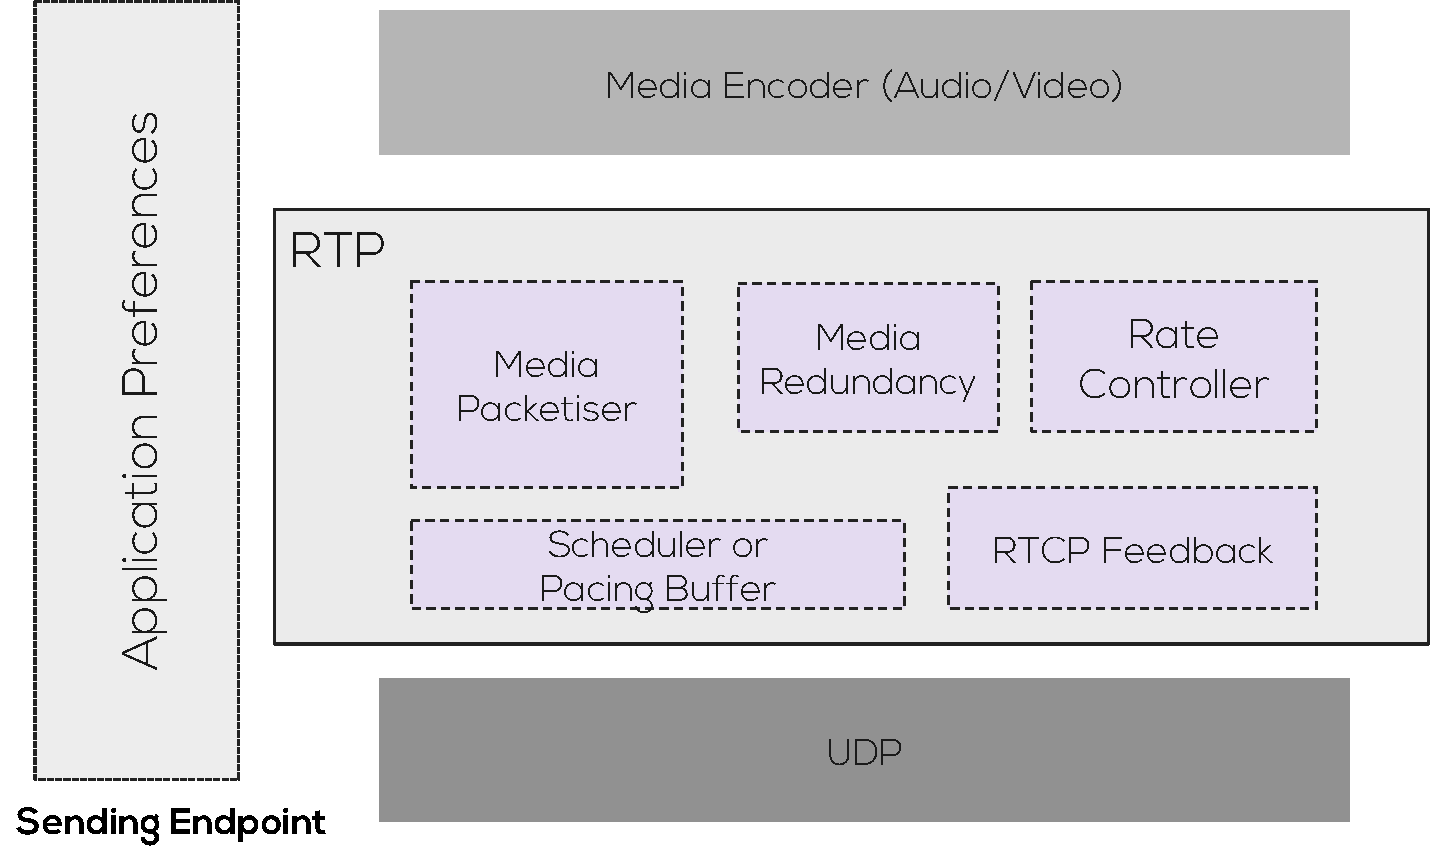
\includegraphics[width=0.66\textwidth]
      {chap4_fig_app_sender}
    }
  }
  \centerline{
    \subfloat[Receiving Endpoint]{
      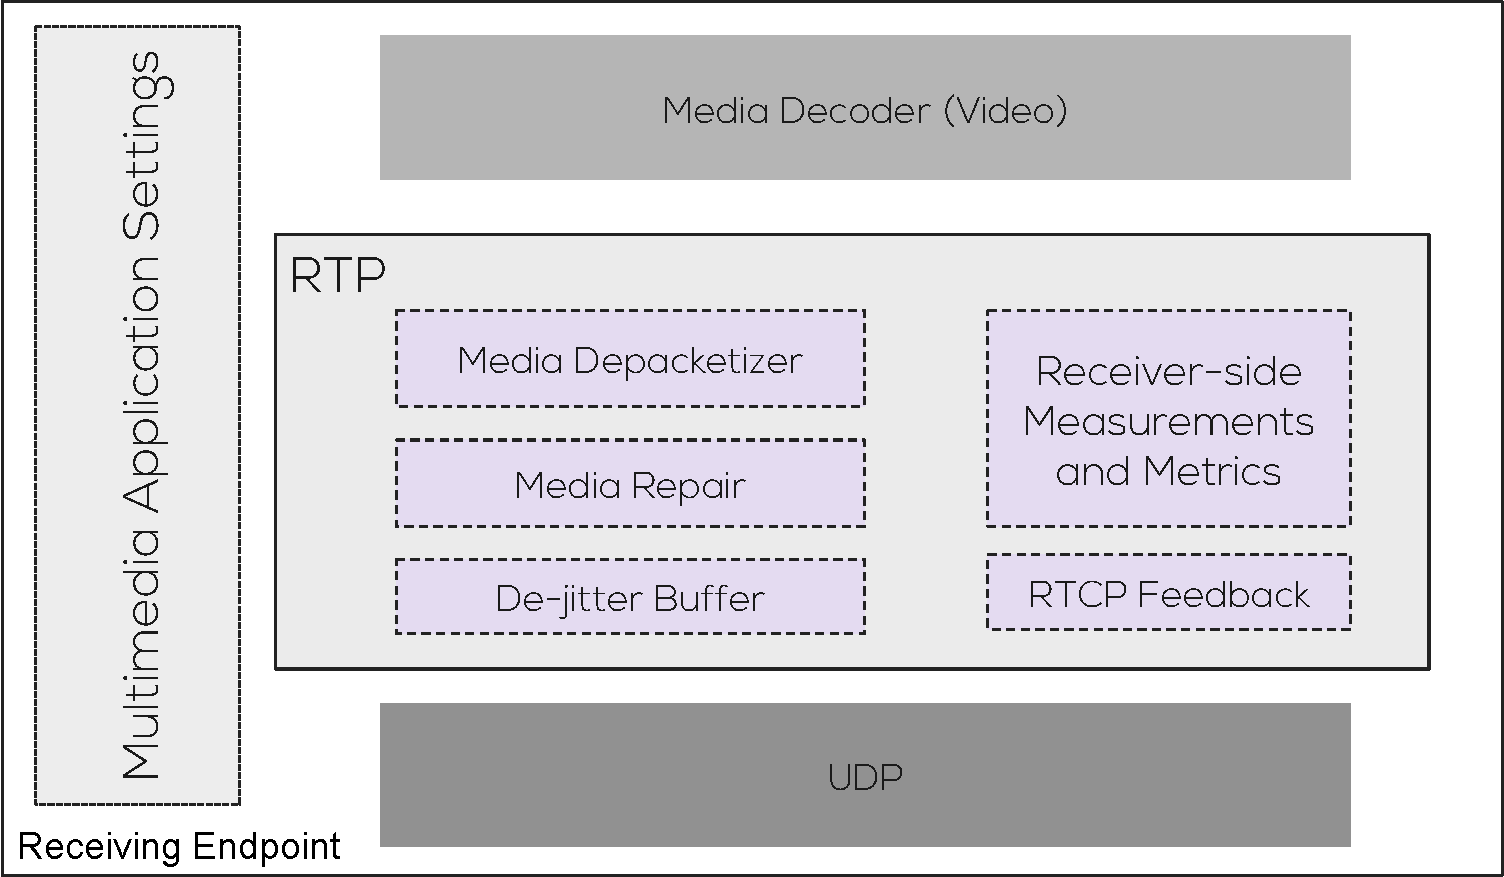
\includegraphics[width=0.66\textwidth]
      {chap4_fig_app_receiver}
    }
  }
  
  \caption{Typical architecture of a multimedia system. a) sending endpoint,
  b) receiving endpoint.}
  \label{fig:4:appint}
\end{figure}

Figure~\ref{fig:4:appint} shows a simplified architecture of a sending and
receiving endpoint; typically, a real-time multimedia application would
contain both these systems and perhaps even two of each for handling audio and
video separately. Figure~\ref{fig:4:appint} (a) depicts the features of the
sending-side RTP stack. The \emph{media packetiser} subsystem receives a video
frame or a series of audio frames from the codec, which it packetises into
RTP. The resulting RTP packets are then passed on to the \emph{media
redundancy} subsystem to be cached if a NACK is received or for producing FEC
packets. Additionally, the RTP packet size and count is sent to the RTCP
subsystem for creating RTCP SR packets. Simultaneously while passing the
packet to the media redundancy subsystem, the RTP packets are sent to the
\emph{pacing buffer or scheduler} subsystem which transmits the packets in a
single burst or trickles them on to the network before the next set of RTP
packets are generated by the media packetiser or codec. The sending endpoint
also routinely generates and receives RTCP packets.

On receiving an RTCP RR packet, it is sent to the \emph{RTCP feedback}
subsystem and onwards to the \emph{rate controller} subsystem. The rate
controller monitors the congestion cues and based on the congestion control
algorithm calculates the new target encoding rate. The codec attempts to
compress the media stream to meet the new target encoding rate in a reasonable
time frame. Figure~\ref{fig:4:appint} (b) depicts the features of the
receiving-side RTP stack. The received RTP packet is put in a \emph{dejitter
buffer} to reassemble out-of-order packets. The dejitter buffer may discard
late arriving packets and it also detects packet loss. Furthermore, the packet
sequence number, size of the packet, RTP timestamp and the reception timestamp
are passed to the \emph{RTCP feedback} subsystem, which routinely generates an
RTCP RR packet and may additionally generate requests for retransmitting
missing RTP packets. This information is also shared with the \emph{receiver-
side measurements and metrics} subsystem, which may generate additional
congestion cues to be sent along with the RTCP RR as RTCP extended reports
(XRs). If FEC packets or other types of repair packets are received, they are
passed on to the \emph{media repair} subsystem which attempts to recover the
missing packets in the dejitter buffer. Eventually, the packets in the
dejitter buffer are sent to the \emph{media depacketiser} where an audio or
video frame is reconstructed and sent to the decoder for playback.


We identify three control loops to implement congestion
control~\cite{Singh:control.loops.api} based on the interaction between the
above components in an multimedia system~\cite{draft.rmcat.app.interaction},

\begin{enumerate}
\setlength{\itemsep}{0pt}

\item \textbf{\texttt{Codec-Sender}}: The codec adapts its encoding rate based
on the feedback from the sender. Unlike elastic traffic, the codec is unable
to produce the expected media rate immediately. Therefore, the rate-controller
needs to take into account the timeline in which the codec produces the new
rate.

\item \textbf{\texttt{Sender-Network}}: The sender packetises media frames and
sends them over the network to the receiver. The sender may however pace the
fragmented frames on to the network instead of sending them in a single
burst. It also collects feedback messages from the receiver that may contain
congestion cues (i.e., variation in RTT, indication of lost or discarded
packets, goodput, jitter, etc.).

\item \textbf{\texttt{Receiver-Sender}}: The receiver has a playout buffer of
media data waiting to be decoded and rendered, discarding packets that arrive
late for playout, and attempting to conceal the missing packets from the
observer. The receiver also monitors the media flow for packet losses,
variation in jitter, receiver rate, goodput, etc. and reports these to the
sender to act upon.

\end{enumerate}

If an endpoint detects congestion rapidly, and the end-to-end path latency is
sufficiently low so that this information can be communicated quickly, it is
possible to change the encoding rate promptly to meet the variation in the 
end-to-end path capacity. However, in practice, this is not always possible because
\textbf{a)} it may take multiple reports or data packets to detect congestion, and
\textbf{b)} after detecting congestion, it takes at least a one-way delay (OWD)
amount of time for the receiver to report it.


\section{Congestion Cues}
\label{fw.cues}

Congestion control algorithms rely on cues to detect congestion. These cues
are detected either by the sender, receiver, or by an intermediary router. The
endpoint observes the congestion along the path and accordingly adapts the
sending rate upon receiving the congestion cues. 
Some common congestion cues are listed below:

\begin{itemize}
\setlength{\itemsep}{0pt}

\item \textbf{\texttt{Losses}}: occur when intermediate routers drop packets
from their queues (\emph{congestion loss}), or due to contention, interference
or fading on wireless link (\emph {bit-error loss}). Losses are inferred at
the receiving endpoint by gaps in RTP sequence numbers. Typically, a dejitter
buffer is used to reorder out of order packets and the fraction packet loss is
calculated at the end of each reporting interval.

\item \textbf{\texttt{Discards}}: packets that arrive too late at the receiver
to be decoded or played back may be discarded by the receiving endpoint. These
late-arriving packets are discarded by the receiver even though they are
received because packets with higher \textit{timestamps} have already been
passed to the decoder for playback. The fractional loss in the standard RTCP
RR does not identify these discarded packets as lost, hence they need to be
reported in an RTCP XRs.

\item \textbf{\texttt{Sending rate, receiver rate and goodput}}: are measured
at the sender, the receiver and at the decoder, respectively. Typically, the
sending rate is the rate at which the media bit stream is generated by the
encoder. If packets are lost in the network, the receiver rate is lower than
the sending rate. Or if duplicate packets are received, the receiver rate is
higher than the sending rate. Lastly, if packets are discarded after arrival
or dropped by the decoder, the goodput will be lower than both the sending
rate and receiver rate. Hence, goodput represents the actual playback bit rate
or the bit rate of the rendered bit stream.

\item \textbf{\texttt{One-way delay (OWD)}}: is a combination of
\emph{propagation}, \emph{queuing}, \emph{serialisation} and \emph{processing}
delay. Propagation delay is calculated from the ratio of the physical length
of the interconnected link and the propagation speed over the specific
medium\footnote{Usually, propagation speed is a fraction of the speed of light
($0.5$c-$0.8$c).}. The serialisation delay is the time taken to send a
complete packet on to the communication channel (link) and is a function of
the link rate and the packet size. The processing delay is the time taken for the
router to determine the next hop or the destination of the packet. Lastly,
when multiple packets are received, the router queues them and transmits them
one by one. Having large-sized buffers in the router causes \emph{buffer-bloat}
\cite{gettys:bufferbloat} and increases the overall one-way delay.
However, measuring one-way delay is difficult because the clocks at the
endpoints are normally not synchronised; instead, the endpoints rely on RTT
measurements for congestion control.

%In a multihop environment, these delays are calculated per hop.

\item \textbf{\texttt{Round trip time (RTT)}}: is the time taken for a packet
to go from the sender to the receiver and then back. In RTP, it is calculated
with the collaboration of sending RTCP SRs and receiving RTCP RRs. In
interactive multimedia, the media flows in both directions, so the one-way
delay (OWD) is approximated as half of the measured RTT. Observing the changes
in RTT provides an indication of congestion and smoothing the RTT
(averaging over a short interval) protects against over-reacting to the subtle
changes in RTT.

\item \textbf{\texttt{Packet delay variation and packet inter-arrival time}}:
packets may arrive at different times due to route changes, or congestion at
the bottleneck link causes jitter. Endpoints detect jitter by comparing the
send or media generation timestamps with the receiving timestamps. The
variation in inter-arrival time may be used to infer congestion.

%\item \textbf{\texttt{Adaptive playout time or Size of Receiver buffer}}:

\end{itemize}

To pick the right congestion cue, an algorithm developer should consider the
following: the type of media stream (audio or video), the expected packet or
frame rate, typical MTU size, interdependence of the streams (audio/video
sync, multi-view video), whether the congestion controller knows the operating environment (Internet-scale, 
low-delay local area deployment, heterogeneous environment with a mix
of wired and wireless links) and the application requirements (audio preferred
over video or vice versa).

Another aspect to consider when picking congestion cues is the the monitoring
duration to identify congestion, i.e., either over a \emph{long-term} (order
of seconds or minutes) or a \emph{short-term} (order of 100\,\emph{ms} or a
few seconds). For example, jitter is measured on a per-packet basis, but
reported over a longer measurement interval (to filter for noise and
transience). In contrast, packet losses, discards, etc. are measured over a
shorter interval so that the sender can react to these immediately.

\section{Congestion Reporting Frequency}
\label{fw.freq}

Normally, congestion control requires a tight control loop, which means that
the receiving endpoint should be able to provide feedback at very short
intervals (at least once per RTT). Hence, the design of a congestion control
algorithm needs to be aware of the limits on the timing of the feedback. For
example, in TCP, the receiver sends an \emph{acknowledgement} packet in
response to every packet (or every few packets) it receives, whereas RTCP
encourages infrequent feedback and specifies an upper-bound on the fraction of
the session media bit rate that the feedback packets can use\footnote{The
specified feedback rate is 5\,\% for each multimedia session.}.
\cite{draft.rmcat.feedback} discusses three options for the short report
intervals,

\textbf{\texttt{Per-packet feedback report}}: sends RTCP feedback every time
the endpoint receives a packet. For low bit rate media sessions (e.g., audio
streams), this would be quite difficult to achieve because the size of the
feedback packet would be comparable to the size of the media packet, i.e., the
feedback bit rate would larger than the 5\,\% fraction specified for it. If an
endpoint receives packets in a burst or at very short time intervals, the
endpoints will not be able to meet the timing requirements for per-packet
feedback because the RTCP timing interval calculation has a randomisation
factor to avoid synchronising feedback from multiple endpoints.

\textbf{\texttt{Per-frame feedback report}}: sends RTCP feedback every time
the endpoint receives a complete frame. This is mainly applicable to video
where a single video frame would be fragmented into multiple packets because
the frame size exceeds MTU size. Typically, an average size of an RTCP packet
size in a two-party call is $156$-$176$ bytes\footnote{The packet breakdown in
bytes is: UDP=16, IPv4=20 or IPv6=40, RTCP=8, SR=20, RR=24, SDES=28, one or
more XR blocks is 20 bytes each.}. For a 30 FPS bidirectional video stream, the
$rtcp\_bw \approx$ 75\,\emph{kbps}, which requires the media session bit rate
be set to a value higher than 1.5\,\emph{Mbps}. Consequently, it would not be
possible to perform per-frame for sessions with lower media rates. It should
be noted that the requirements for the media session bit rate needs to be 
re-calculated if the number of participants change, the number of reported
blocks change, or the frame rate changes.

\textbf{\texttt{Per-RTT feedback report}}: sends RTCP feedback at regular
intervals based on the RTT estimate. The requirement for the media session
rate would be lower, if the RTT is higher than the frame inter-arrival time.
The calculation of the RTCP interval for the per-frame still applies, except
that the frame rate is replaced by the RTT estimate.

To summarise, picking longer RTCP feedback intervals requires a lower media
session bit rate, hence it increases the possibility of applying the same
congestion control to a larger operating area (in terms of session media
rates).

\section{Framework for Classifying Congestion Control}
\label{fw.fw}

A rate-control or congestion control algorithm relies on congestion cues to
pick a new sending rate. These cues are either observed at the receiver or by
intermediaries monitoring the flow, or are aggregated by a
third-party\footnote{A system outside the signalling or media path} or a
super-peer in an overlay network. Consequently, these observed cues need to be
signalled back to the sender which will perform congestion control. We classify
these congestion cues as a combination of \emph{where are they
measured/observed?}, and \emph{how is the sender notified?} For each, there are
two options: In-path and Off-path \emph{sources} and In-band and Out-of-band 
\emph{signalling}~\cite{Singh:PhDFw}. In-path congestion cues are measured
by the receiver or by intermediaries along the path. Off-path congestion
cues are reported by devices outside the media path (congestion maps,
overlays, etc.). The combination forms four cases which are visualised in
Figure~\ref{fig:4:fw}.

\begin{figure}
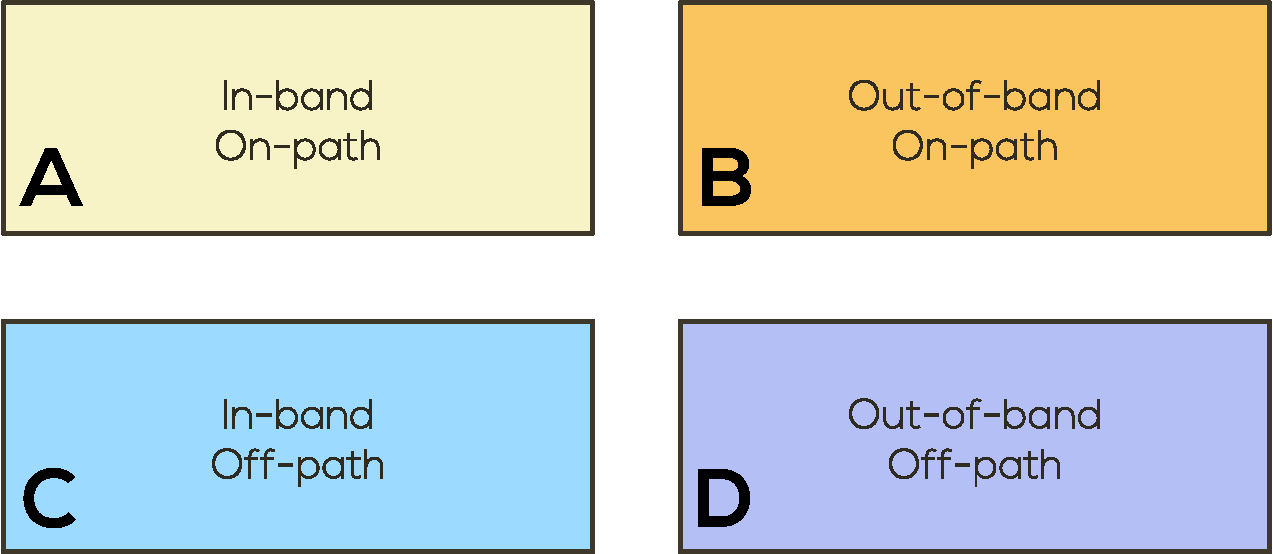
\includegraphics[width=0.9\textwidth]{chap4-fig-fw-outline}
\caption{Framework for classifying congestion control~\cite{Singh:PhDFw}.}
\label{fig:4:fw}
\end{figure}

A congestion control algorithm needs to pick one or more measurement point
(picking multiple adds to the feedback overhead) and then choose a method
to signal it to the sending endpoint. The algorithm can choose to report it in-band by
encapsulating the cues, either by piggybacking them on the endpoint's own media
packets as RTP header extensions (this adds to the header overhead of a media
packet) or as RTCP extension blocks (see section~\ref{fw.freq} for details on
feedback frequency). Or the congestion control algorithm can choose to signal
the cues out-of-band, i.e., re-use the signalling path (e.g., SIP, XMPP) or
setup an alternate signalling path (e.g., HTTP or websockets). The following are
examples for each category in the framework:

\textbf{\texttt{A) In-path, In-band}}: The congestion control algorithm in
this case relies on the cues reported in an RTCP feedback from the receiver.
For example, TFRC using information in RTCP RR, TFRC using additional loss
reported by ECN markings, Temporary Maximum Media Stream Bit Rate Request
(TMMBR), Receiver Estimated Max Bit rate (REMB).

\textbf{\texttt{B) In-path, Out-of-band}}: The congestion control algorithm
relies on the cues reported in the signalling channel; for example, RTSP implements
a \emph{Speed} parameter to vary the transmission rate, or 3G base stations announce
the new rate when capacity changes due to cell-loading or handover.

% announcing bandwidth in the SDP at the start of the session (instead of
% starting at a low media bit rate) for rudimentary congestion control,

\textbf{\texttt{C) Off-path, In-band}}: The congestion control algorithm
relies on reports from multiple in-band sources; for example, in Multipath
RTP, congestion on one path causes a change in the fractional distribution of
traffic on each path.

\textbf{\texttt{D) Off-path, Out-of-band}}: The congestion control
algorithm relies on third party sources such as receiving bandwidth or
congestion notifications from congestion maps, bandwidth lookup services,
super-peers and overlays.

% monitoring: long-term, short-term

% Additionally if the cue reliably
% describes the onset of congestion (\emph{knee}) or the collapse
% (\emph{cliff}).

% \begin{figure}[!h]
% 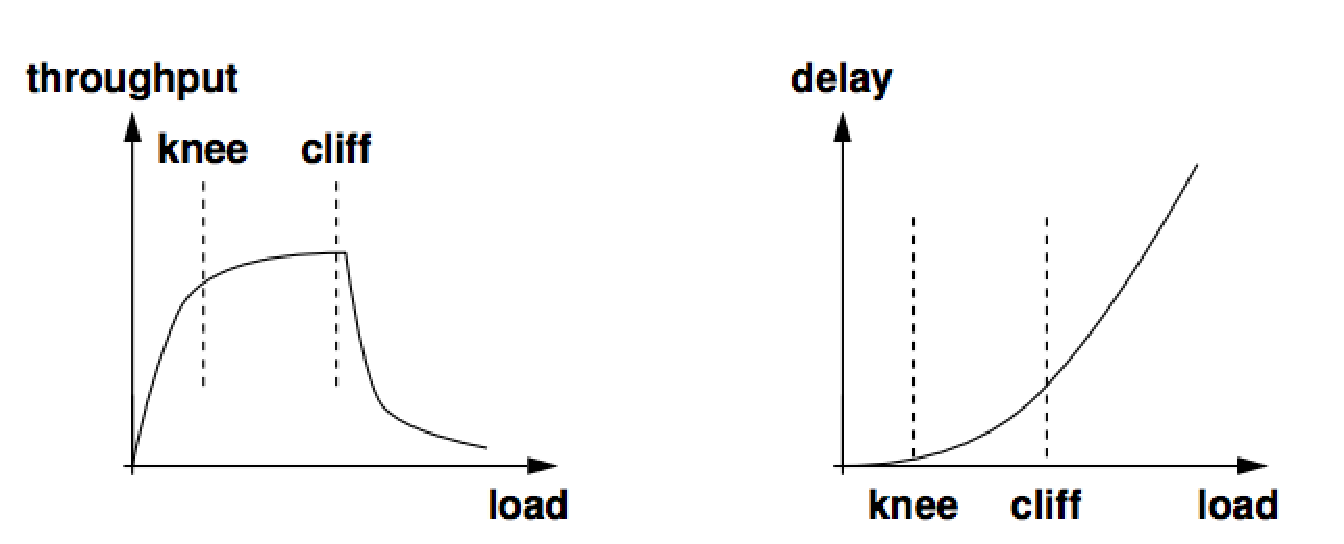
\includegraphics[width=\columnwidth]{chap4-knee-cliff}
% \caption{Shows the variation throughput and delay with increasing network load.}
% \label{fig:4:knee}
% \end{figure}

\section{Types of Video Frames in Interactive Multimedia}

In this subsection we briefly discuss codec design related to interactive
multimedia and limit the discussion to H.264 and VP8 codecs, however it may
apply to other modern codecs as well. Both H.264~\cite{h264} and
VP8~\cite{rfc6386} internally decompose a video frame into square blocks
called \emph{macroblocks}. The macroblock coder typically uses inter frame
prediction with motion compensation for compression. Further, the codec design
is conceptually divided into a Video Coding Layer (VCL) and a Network
Abstraction Layer (NAL). The VCL takes a complete uncompressed frame and
outputs slices, which is a group of one or more macroblock. The NAL
encapsulates these slices into packets, which can be transmitted over IP
networks.

H.264~\cite{h264} has three types of frames: I-, P-, and B-frames. The I-frame
is an \emph{intra-coded frame}, which does not dependant on any previous frame
and is in effect like a compressed static image. While the other two types of
frames hold only parts of the image, are hence smaller in size but depend on
other frames to be successfully decoded. A P-frame is a \emph{predictive coded
frame}, it encodes only the changes from the previous frame. A B-frame is a
\emph{bipredictive coded frame}, it encodes the changes from the previous and
next (future) frame. In interactive multimedia, the use of B-frames is
avoided because depending on future frames introduces unnecessary delay in
transmission. Therefore, all the algorithms proposed in this thesis use just
I- and P-frames during media encoding.

VP8~\cite{rfc6386} has two types of frames: intraframes and interframes.
Intraframes\footnote{Also known as I-frames or key frames in H.26x codecs} are
compressed without references to any previous frames and can therefore be
decoded by an endpoint without receiving any other frames. Essentially, the
decoder resets its internal state and stops any previous errors from
propagating because of loss of intermediate frames. Interframes\footnote{Also
known as P-frames or dependent frames in H.26x codecs} are encoded with a
reference to previous frames up to the most recent intraframe. A loss or
corruption of a single interframe will affect the decoding of all the
subsequent dependent interframes i.e., rendering errors will occur, until a
new intraframe is received. To overcome this limitation, VP8 introduces a
concept of golden frames or alternate reference frames, wherein interframes
can refer to not only the most recent interframe but also to previous
intraframe.


\section{Congestion Control Evaluation}
\label{fw.cc.eval}

% We need to define a set of requirements in order to design a congestion
% control algorithm for multimedia streams. Later these requirements are used as
% a checklist to evaluate the suitability of the proposed algorithms.

Real-time interactive communication differs greatly from \emph{elastic}
traffic because the sender generates media packets in real-time and expects it
to be delivered in hundreds of milliseconds, and the receiver consumes the media
packets almost immediately, hence late-arriving packets are useless.
Additionally, real-time communication systems are able to tolerate some amount
of packet loss and adapt the media rate over a fairly large range.
\cite{draft.rmcat.req} lists a set of requirements for RTP-based interactive
multimedia sessions; these requirements form the basis of the guidelines
described in~\cite{draft.rmcat.evaluate}. In~\cite{draft.rmcat.eval.test}, we
define a catalogue of \emph{traffic flows} traversing through a \emph{network
topology} with varying \emph{link characteristics} and diverse \emph{queuing}
strategies. By picking one feature from each category, we
construct scenarios to evaluate the performance of the congestion control. The
evaluation scenarios are built using the following components: network
topology, link and router characteristics.

The difference between testing in real-world deployments and in simulations is
also important to consider, mainly in terms of the accuracy of RTT
measurements which impacts delay-based algorithms (e.g., TFRC). Time-slot-driven
simulation systems, such as \emph{ns-2}~\cite{ns2}, have accurate timing that
is not representative of real-world systems. Testbeds usually use
dummynet~\cite{Carbone:2010p3502}, NetEm~\cite{netem}, or packet traces to
emulate the variation in link capacity, latency, intermediate router queue
length, and packet losses. 

It is also possible to use actual machines placed at geographically distinct
locations and send media traffic between them; however, in this case, it is
not possible to run a controlled experiment anymore because of the varying
amount of cross-traffic generated by other hosts in the network. Usually the
last step in the evaluation process involves deploying the congestion control
algorithm on several (thousands of) endpoints and showing that it behaves as
described without breaking anything on the network (i.e., causing a congestion
collapse).

\subsection{Network flows}

In this section, we describe typical test scenarios for evaluating congestion
control algorithms. These test scenarios are not supposed to be exhaustive
but show the applicability range of the algorithm.

\begin{enumerate}
\setlength{\itemsep}{0pt}

\item \textbf{\texttt{Single media flow on an end-to-end path}}: This scenario
describes the best case, wherein the network puts each flow identified by its
5-tuple (protocol, source and destination IP address, source and destination
port numbers) in its own queue, thus the flow using the proposed congestion
control algorithm does not encounter any cross-traffic.

\item \textbf{\texttt{Single media flow competing with multiple similar
flows}}: In this scenario, the flow using the proposed congestion control
algorithm competes with multiple flows using the same congestion control algorithm
(i.e., all flows are interactive multimedia).


\item \textbf{\texttt{Single media flow competing with multiple TCP flows }}:
In this scenario, the flow using the proposed congestion control algorithm
competes with TCP flows. These maybe \emph{short} TCP flows representing
common web-traffic patterns or \emph{long} TCP flows depicting bulk transfers
(e.g., large file downloads).

\end{enumerate}

% In Section~\ref{rg.title}, we describe the network traffic scenarios to
% evaluate the proposed congestion control algorithms, namely, when the flows
% are a) alone, b) competing with self-similar flows, and c) competing with TCP
% flows (short-, long-lived) on a bottleneck link.




\subsection{Link characteristics}

The link characteristics can be broken down into the following categories:
capacity, latency, and loss. The capacity of a link mainly varies in wireless
networks (for example in 3G, LTE, WLAN, etc). In Wireless LAN (WLAN) networks,
the capacity varies depending on the density of nodes using the network. The capacity in
mobile networks (e.g., 3G, LTE) fluctuates for each user because of fading,
interference, mobility, handover, cell loading, etc. The latency of a link
is measured as the propagation and serialisation delay. Queuing delay is based on the
queue size of the router and hence, is a router characteristic. Latencies between
nodes typically vary from a few milliseconds to a few seconds. Commonly used
values are: LAN (very low delay, <1\,\emph{ms} ), low delay (<40\,\emph{ms}),
trans-continental (>100\,\emph{ms}), or satellite links (>500\,\emph{ms}).
Packet losses are modelled using the Gilbert-Elliott
Model~\cite{gilbert1960capacity, elliott1963estimates} or by packet
traces~\cite{ellis:2011:dataset, 3gppSim}.


\subsection{Router characteristics}

 % Queue-size and Queue type.

Apart from managing packet routing, a router also manages congestion; when a
packet arrives at a higher rate than it can be processed, the router queues the
packet. The routers then use \emph{priority queuing}, \emph{fair queuing}, or
\emph{weighted fair queuing (WFQ)}~\cite{rfc4594} to decide which traffic
class to transmit or drop packets from during congestion. When congestion
occurs within the same traffic class, the router discards packets using
\emph{tail drop}, \emph{Random Early Detection (RED)}~\cite{Floyd:RED}, or
\emph{Weighted Random Early Detection (WRED)}.

We describe the queue sizes as a function of time, i.e., it is the depth of
the queue or the amount of time the packet will remain in the queue before it
is discarded. However, in practice, the queue size is measured in number of
packets. We convert the queue depth (measured in time) to queue length (number
of packets, MTU is typically 1500 bytes) using:

\begin{equation*}
  \mathrm{QueueSize}_\mathrm{packets} = 
    \frac{\mathrm{QueueSize}_\mathrm{sec} \times
    \mathrm{Throughput}_\mathrm{bps}}{\mathrm{MTU} \times \mathrm{8}}
\end{equation*}

For example, a router with a throughput of 1\,\emph{Mbps} and a 1\,\emph{s} queue depth would be
capable of handling 83 packets (queue length). A 100\,\emph{ms}
queue depth may represent a short queue, while a 10\,\emph{s} queue depth represents
a buffer-bloated queue.

\subsection{Network topology}

We should run different types of network topologies to evaluate the
performance of congestion control. Depending on the amount of cross-traffic,
the bottleneck link will move from one node to another in the network. Also,
the bottleneck in each direction may be different due to the asymmetry of
access links. Additionally, the varying capacity of the access link (e.g., in
wireless environments) may be the bottleneck.


\begin{figure}
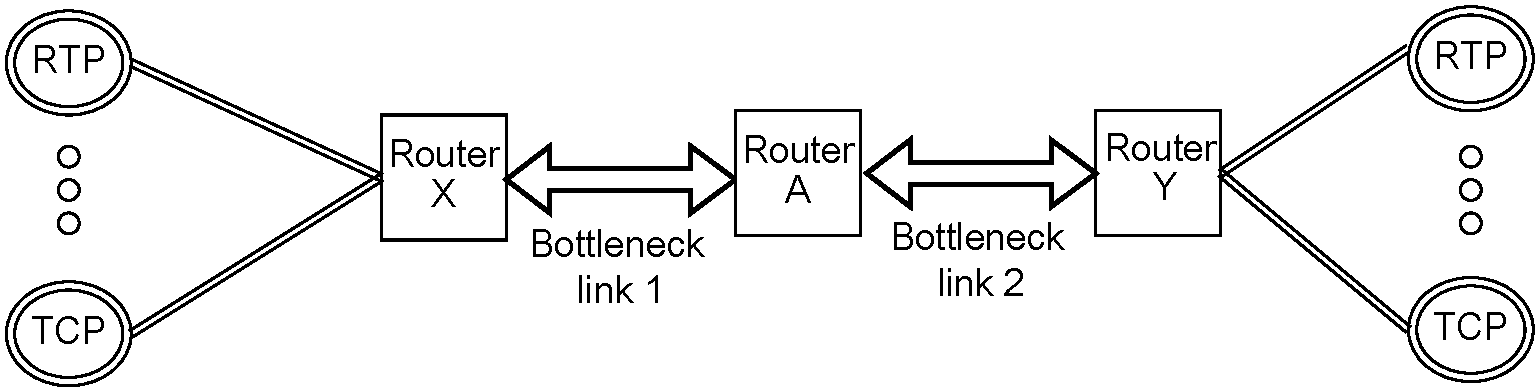
\includegraphics[width=\textwidth]{chap4_fig_sim_topology}
\caption{Typical network topology for evaluating congestion control consisting
of traffic flows (evaluating flow and cross traffic), links and routers.}
\label{fig:4:topology}
\end{figure}


Figure~\ref{fig:4:topology} shows an example of the evaluation setup. This
topology is commonly called the \emph{dumb-bell} topology. Another common
topology is \emph{parking lot}, which uses multiple bottlenecks instead of a
single bottleneck; however, both use common concepts.


To define a scenario, we need to choose the following: the type of cross-
traffic (self-similar, short- or long-lived TCP), the characteristics of the
cross traffic (e.g., duration), the characteristics of the edge routers
(Router X and Y) and the impairments in the network. Lastly, we have to
measure and analyse the performance of the multimedia system.


\subsection{Our Evaluation Setup}

Our research made use of the network simulator (\emph{ns-2})~\cite{ns2} or a
testbed made up of real-machines. The individual link characteristics in the
testbed were either controlled by NetEm~\cite{netem} or by
dummynet~\cite{Carbone:2010p3502}; the intermediate machines that ran
NetEm/Dummynet ran kernels re-compiled at 1000Hz for better performance. The
endpoints typically ran stock Linux, such as Ubuntu 10.04 or 12.04. In some
cases, we used bandwidth and packet loss traces provided by
3GPP~\cite{s4.eval.bitrate} or collected them ourselves~\cite{sharmistha-thesis}. 
Additionally, we ran some tests between machines in Helsinki and the
Amazon data centers located in Virginia (US-EAST) and Ireland. The details of the
individual test scenarios are discussed in detail in the associated scientific 
papers.

\subsection{Metrics for Congestion Control}
\label{subsec.metrics}

In this section, we introduce metrics for evaluating congestion control
algorithms. Multimedia application observe the congestion cues, and react to
the changes in the cues, by modifying the encoding/sending rate to match the
available end-to-end bit rate. The sender's goal is to minimise losses at the
receiver while maintaining a stable throughput. Losses are caused by
congestion or by bit-errors and are detrimental to the perceived video quality. Although,
real-time communication is tolerant to a small amount of losses, bursty loss
should be avoided. 

% Bit-errors are due to the physical properties of the network and cannot be
% predicted ahead of time. Congestion losses are due to over-utilization of the
% links and may cause long delays or congestion-induced drops at the router.



\begin{figure}
\centering
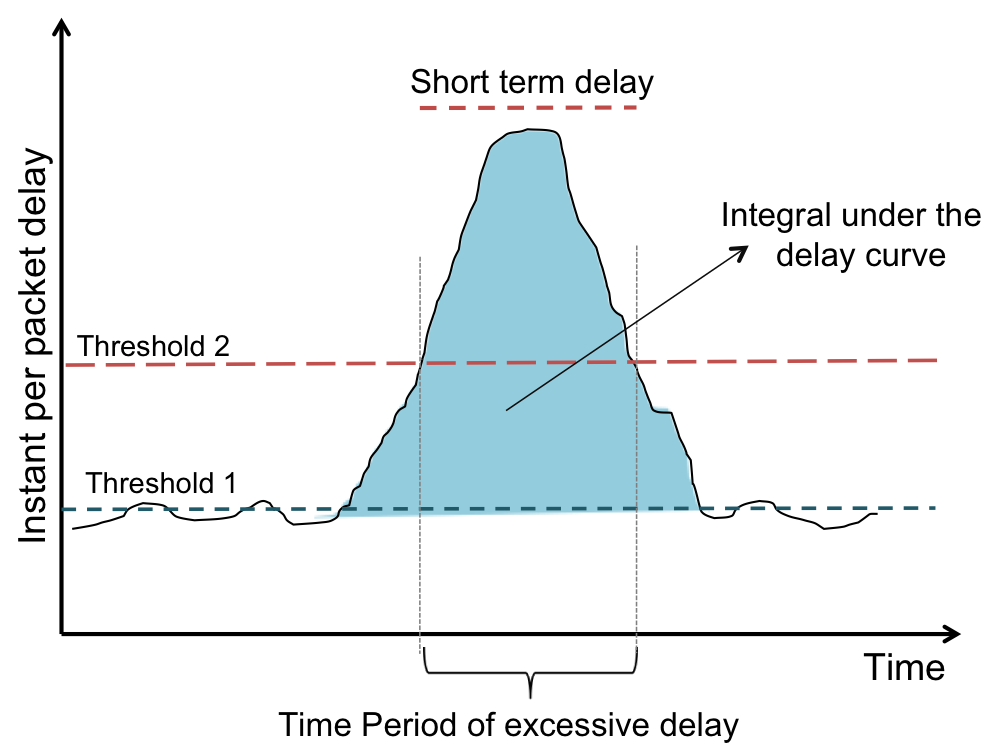
\includegraphics[width=0.75\textwidth]{chap4_fig-perf-metrics}
\caption{Metrics for congestion control.}
\label{fig:4:rc_model}
\end{figure}

Figure~\ref{fig:4:rc_model} schematically shows the instant per-packet delay
over time observed at the receiver. The sender reacts to the changes in the
available path bit rate. Exceeding the available path bit rate may lead to a
temporary increase in per-packet delay until the rate adaptation measures take
effect and, optionally, to packet losses if the queue capacity is exceeded.

For the delay, we define three values:
\begin{itemize}
\setlength{\itemsep}{0pt}

\item \textbf{\texttt{Threshold 1}} refers to the mean one-way delay observed
under normal operating conditions; this value may be defined statically
according to expectations for a certain environment, or determined
dynamically. This reflects the mouth-to-ear or camera-to-eye delay.

\item \textbf{\texttt{Threshold 2}} defines the maximum acceptable one-way
delay for a packet after which the rendering of the received media packet is
no longer meaningful. Packets arriving later than threshold 2 will be
discarded.

% Threshold 2 may be, e.g., 100-500ms for video, since the human eye
% is more tolerant to video glitches~\cite{s4.eval.fw}.

\item The \textbf{\texttt{short-term delay peak}} reflects the maximum delay
peak encountered during a congestion control operation. This may be either
caused by the appearance of cross-traffic on the bottleneck link or due to
congestion resulting in self-inflicted delay.

\end{itemize}

For losses, we consider two values:
\begin{itemize}
\setlength{\itemsep}{0pt}

\item \textbf{\texttt{Packets lost}} in the network due to bit errors and/or
increased queue lengths or overflows (e.g., caused by drop-tail or RED queue
management).

\item \textbf{\texttt{Packets discarded}} at the receiver because their
arrival delay violated threshold 2.

\end{itemize}

Additionally, we measure the instantaneous and average encoder rate, receiver
rate and goodput. The instantaneous rate is calculated at 1 second intervals. The
Average Bandwidth Utilisation (ABU) is the ratio between the instantaneous
goodput (or encoding, receiving bit rate) and the instantaneous channel
capacity at 1 second intervals. An ABU larger than 100\,\% represents over-utilisation 
and the duration over which it is over 100\,\% signifies the congestion period.


Peak Signal-to-Noise Ratio (PSNR) is the ratio between the maximum possible
power of a signal and the power of a noisy signal. The maximum power signal is
presumed to be the original signal, while the noisy signal is the received data
signal that has undergone the cycle of compression-transmission-decompression.
While PSNR is the most widely used objective video quality metric, it does not
perfectly correlate with perceived visual quality due to the non-linear
behaviour of the human visual system~\cite{itu-t-j247}. Another criticism
against PSNR is that it does not incorporate time in its calculation. Despite
its shortcomings, we use PSNR as a yet another indicator for measuring the
performance of congestion control. Recently, a number of new techniques were
proposed for measuring video quality more accurately than PSNR: 
Video Quality Metric (VQM)~\cite{itu-t-j144}, and Perceptual Evaluation 
of Video Quality (PEVQ)~\cite{itu-t-j247, itu-t-j341}, but these metrics are not 
used in this thesis and will be adopted in the future work.

% It has been observed that the pictorial quality perceived by the human visual
% system is also affected by the overall general impression of the viewed video
% stream. In addition, recent studies have shown that human visual system awards
% higher response to more salient image locations and
% features~\cite{Li02asaliency, Ong:2006p3066}.


\section{Circuit Breakers for Unicast RTP Sessions}

If congestion control is not implemented by multimedia applications, they can
cause severe congestion in the network, especially if high data rate media
traffic is sent over low-capacity networks. This can not just disrupt the
multimedia's quality of experience but also other applications on the network.

We are developing a circuit breaker algorithm that can work with unmodified
RTP applications to determine when these non-adaptive multimedia
applications are causing excessive network congestion and force them to cease
transmission. We envision that the congestion control algorithms for
multimedia standardised in the IETF will need to work inside the envelope of
this circuit breaker algorithm~\cite{draft.rmcat.evaluate}, i.e., a multimedia
application implementing congestion control should not trigger the circuit
breaker. Consequently, the circuit breakers cannot be too aggressive in
terminating media flows because it should allow sufficient time for the
congestion control algorithm to monitor and respond to congestion cues.

The circuit breaker algorithm in the short term will serve as a policer,
during which time the congestion control algorithm is developed. Developing
standard congestion control algorithms for unicast RTP-based interactive
multimedia applications is expected to be a multi-year process in the IETF.
Therefore, the development of the circuit breaker is on a tight schedule, to
be ready for inclusion in the initial roll-out of the WebRTC (Web-based 
Real-time Communication) framework~\cite{jennings:2013:webrtc} in web browsers.

\subsection{Circuit Breaker Design}
\label{fw.cb.design}

The RTP circuit breaker algorithm relies on the basic feedback mechanisms
defined in the RTP Control Protocol (RTCP)~\cite{rfc3550}. That is, it solely
uses the information available in the RTCP Sender Report (SR) and Receiver
Report (RR) packets to detect if the flow is overusing the capacity or causing
congestion.

The congestion indicators considered for implementing circuit breakers are: 1)
the network \emph{round trip time} (RTT) calculated using timing information
in RTCP SR and RR packets, 2) the \emph{jitter} estimated by the receiver over the
last reporting interval, and 3) \emph{fractional packet loss} and \emph{cumulative
loss} reported by the receiver during the last RTCP interval. These
indicators unfortunately only provide a limited insight into the behaviour of
the network and cannot be used as strong signals for a circuit breaker.

Variation in RTT is used as a congestion indicator in delay-based congestion
control algorithms. Additionally, some algorithms use RTT estimates to
configure connection timeouts. In RTP/RTCP, the RTT is estimated infrequently
because the feedback intervals are rather long, making it difficult to detect
the cause in variation of delay. Likewise, variation in jitter can indicate a
transient network congestion but does not provide a strong enough signal to implement
a circuit breaker. On the other hand, loss is a strong indicator of congestion
in networks where packet losses predominantly occur due to queue overflows, and
is a less accurate indicator where packet loss occurs due to bit-error
corruption (e.g., wireless and mobile links). Therefore, we base the circuit
breaker conditions on packet losses. 

\begin{enumerate}
\setlength{\itemsep}{0pt}

\item \textbf{\texttt{Media Timeout}}: An endpoint is sending media data but when
the receiver reports a non-increasing \emph{Highest Sequence Number} (HSN) for
two consecutive RTCP intervals, the flow is terminated.

\item \textbf{\texttt{RTCP Timeout}}: An endpoint is sending media data but if it
receives no RTCP RR for three consecutive RTCP intervals, the flow is
terminated.

\item \textbf{\texttt{Congestion}}: An endpoint is sending media data and if it
receives RTCP RRs indicating fractional packet loss, it calculates the TCP-friendly 
rate and compares it to the sending rate. If the sending rate exceeds
the TCP-friendly rate by a factor of 10 for two consecutive RTCP intervals,
the flow is terminated.

\end{enumerate}

Full details of the RTP circuit breaker algorithm is specified
in~\cite{draft.rtp.cb}, which is a work in progress and covers various
deployment cases such as multiple media sources, impact of shorter-than-standard 
reporting interval, deployment of Explicit Congestion Notification
(ECN), etc.

In \citepub{c:cb}, we apply these circuit breaker conditions to non-adaptive
RTP media flows deployed on ADSL and cable modem links. Such flows typically
do not implement congestion control at this time, and are likely to cause
congestion if deployed on the Internet. We carried out a series of experiments
based on real-world traces and on a testbed emulating real-world conditions.
Our results show that the proposed RTP circuit breaker performs well,
triggering in cases of bursty loss and in sessions that are congesting the
links, and does not trigger in low-loss and non-bursty scenarios.


\begin{figure}
  \centering{
    \subfloat[Non-bursty]{
      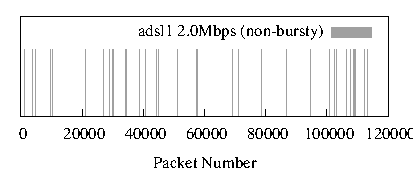
\includegraphics[width=0.66\textwidth]
      {chap4_graph_cb_20090707-1515-barcode}
    } \\
    \subfloat[Bursty]{
      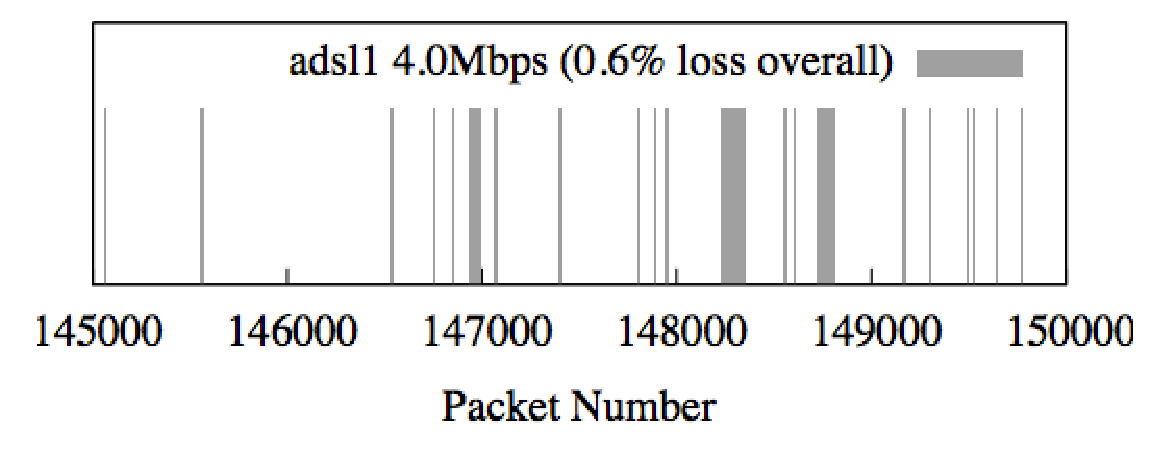
\includegraphics[width=0.66\textwidth]
      {chap4_graph_cb_bursty}
    }
  }
  \caption{Sample non-bursty (a) and bursty (b) packet loss traces.
  The bursty packet triggers the circuit breaker even though the overall
  packet loss ratio is 0.6\,\%.}
  \label{fig:4:bursty}
\end{figure}

\begin{table}
  \begin{center}
    \begin{tabular}{rcc}
    \toprule
      \textbf{Loss Pattern}   & \textbf{Triggered} & \textbf{Did not trigger} \\
    \midrule
             Loss free &   0.0\,\% & 100.0\,\% \\
       Non-bursty loss &   0.0\,\% & 100.0\,\% \\
          Bursty loss  &  11.9\,\% &  88.1\,\% \\
    \bottomrule
    \end{tabular}
    \caption{Sessions triggering the circuit breaker by loss pattern.}
    \label{tab:4:cb_bursty}
  \end{center}
\end{table}

We simulated the RTP circuit breaker performance on $3833$ generated RTCP traces
corresponding to the measurements collected in \emph{dataset-A} and
\emph{dataset-B} of~\cite{ellis:2011:dataset}. Of these, $1626$ traces have no
packet loss, and hence cannot trigger the RTP circuit breaker. The remaining
traces each include at least one lost packet. We categorise the remaining
traces into two categories: those that have non-bursty packet loss, and those
that exhibit bursty loss using the definition of bursty loss
from~\cite{rfc3611} (Figure~\ref{fig:4:bursty} shows representative samples of
the non-bursty and bursty packet loss patterns). The data comprises $1344$
traces with bursty loss and $863$ traces with non-bursty loss.



Table~\ref{tab:4:cb_bursty} shows the fraction of sessions that triggered the
RTP circuit breaker for each of the categories of packet loss. The RTP circuit
breaker did not trigger for sessions without loss; it also did not trigger for
any of the sessions with non-bursty packet loss. However, we observe that the
RTP circuit breaker is triggered more often in sessions that contain bursty
packet loss. 

\begin{figure}[!t]
  \centerline{
    {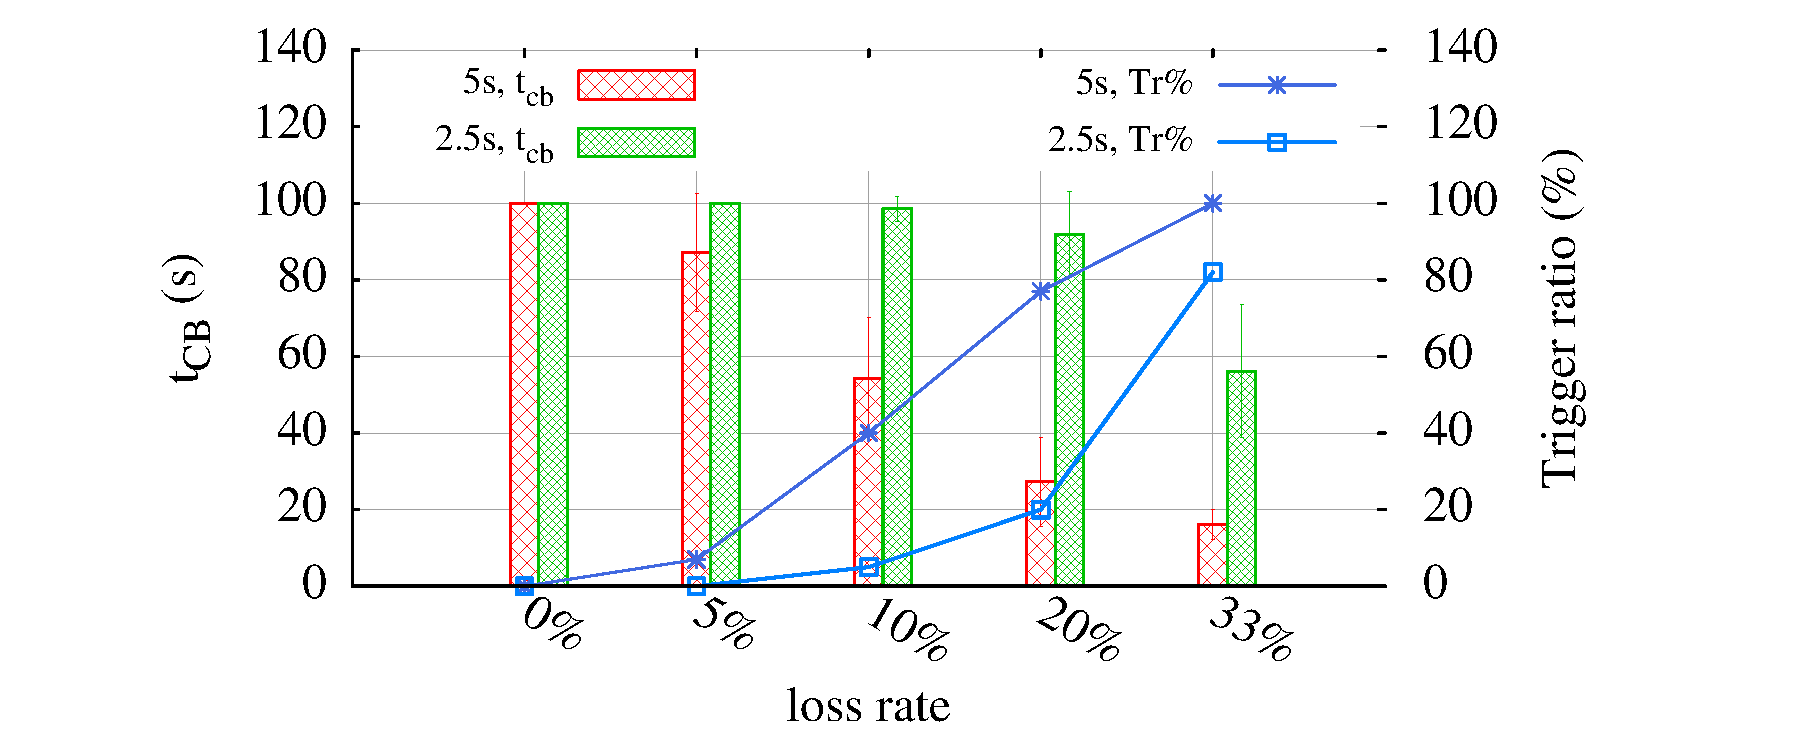
\includegraphics[width=\textwidth]{chap4_graph_cb_cmp_trr_2s}}
  }
  \caption{Impact of using a shorter RTCP interval on the
  circuit breaker. Each scenario was run 50 times and the error bars represent
  the 95\,\% confidence level.}
  \label{fig:4:short-rtcp}
\end{figure}

The circuit breaker conditions trigger mainly due to loss. Figure~\ref{fig:4:short-rtcp} 
shows that the percentage of sessions triggering the circuit breaker
increases with the increase in loss rate. The figure also shows the impact of
the RTCP reporting interval, i.e., by reducing the RTCP interval from 5\,\emph{s} to
2.5\,\emph{s}, fewer sessions are terminated. The endpoints become robust to loss of
feedback packets by sending feedback often and we observe a longer time for
triggering the circuit breaker ($t_{CB}$).

\subsection{Discussion about TCP throughput equations}

In Section~\ref{fw.cb.design}, we described the circuit breaker triggers when
the sending rate exceeds the estimated TCP throughput by a factor of 10. We
can estimate the TCP throughput either using Padhye's full TCP throughput
equation~\cite{padhye1998modeling} or using Mathis's simplified TCP throughput
equation~\cite{mathis1997macroscopic}.

In~\cite{padhye1998modeling}, Padhye \emph{et al.} show that the TCP
throughput for a long-lived TCP Reno connection can be estimated using the
following equation:
\begin{align*}
X_{kbps} = &\frac{8 \times s}{R \times \sqrt{\frac{2*b*p}{3}}+t_{RTO} \times (3 \times \sqrt{\frac{3*b*p}{8}})\times p \times (1+32 \times p^2)}\\
\end{align*}
While Mathis \emph{et al.} in \cite{mathis1997macroscopic} show that under
conditions of low packet loss, Padhye's equation can be simplified to:
\begin{align*}
    X_{kbps} = & \frac{8 \times s}{R \times \sqrt{\frac{p \times 2}{3})}}
\end{align*}
\begin{itemize}
\setlength{\itemsep}{0pt}
{\footnotesize
\item[] \texttt{X is the transmit rate in kbps.}
\item[] \texttt{s is the average packet size in bytes.} 
\item[] \texttt{R is the round trip time in seconds. }
\item[] \texttt{p is the loss event rate, $\forall p \in [0.0, \cdots ,1.0]$.}
\item[] \texttt{$t_{RTO}$ is the TCP retransmission timeout value in seconds, usually set to $\mathbf{4 \times R}$.}
\item[] \texttt{b is the number of acknowledged packets in TCP; typically set $\mathbf{b=1}$.}
}
\end{itemize}
Mathis \emph{et al.} also show that the simplified TCP equation approximates
Padhye's full equation with reasonable accuracy~\cite{mathis1997macroscopic} .


In \citepub{c:cb}, our experiments on residential networks shows that the
simplified TCP throughput equation performs effectively, while using Padhye's
full TCP equation triggers the circuit breaker earlier. The data show that
the full TCP equation tends to be more sensitive to packet loss. In LTE
networks with a combination of a low RTT and high packet loss rate (due to
AQM), the circuit breaker using the simplified TCP throughput equation
does not trigger at all~\cite{Sarker:CB.lte}. However, using the Padhye's full TCP
throughput equation in these cases gives better
performance~\cite{Sarker:CB.lte}. We believe some of this over-sensitivity is
due to averaging packet loss events over long RTCP reporting intervals and the
fact that the RTT is estimated only once in that interval.

Overall, our preliminary results derived from experiments in a testbed,
and simulations based on real-world traces show that
the proposed RTP circuit breaker performs as intended, triggering in the case
of bursty packet loss and not triggering in the low-loss and non-bursty
scenarios. 

% The current analysis is based on measurements done in the UK and
% Finland, while these measurements may be representative of residential links
% in Europe, the infrastructure is likely to differ significantly in other parts
% of the world. Therefore, a wider measurement study of the RTP circuit breakers
% would be desirable.


\section{Summary}

In this chapter, we aimed to classify congestion control cues for real-time
communication based on: \emph{where they are measured?} (by in-path or off-
path sources) and \emph{how they are reported?} (via in-band or out-of-band
signalling). We also describe other fundamental choices needed to implement
congestion control: congestion cues, reporting frequency and circuit-breaker
conditions. Additionally, we describe a basic evaluation suite for measuring
the performance of any proposed multimedia congestion control algorithm;
derivatives of these test scenarios are used to discuss the performance of
congestion control in this thesis.

We specified the circuit breaker algorithm and discuss the performance of the
circuit breaker applied to non-adaptive multimedia traffic. Our results show
that it works as intended, i.e., it provides enough time for a congestion
control algorithm to respond to congestion cues before triggering the circuit
breaker. We also show that the endpoint can slightly vary the sensitivity of
the circuit breaker by choosing between the full and simplified TCP throughput
equation. In the forthcoming chapters, we discuss our proposals for congestion
control in various environments, several of which work within the constraints
imposed by the circuit breaker algorithm.


